\documentclass[a4paper,oneside,14pt]{extreport}

\usepackage[T2A]{fontenc}
\usepackage[utf8]{inputenc}
\usepackage[english,russian]{babel}

%\usepackage[left=30mm, right=20mm, top=20mm, bottom=20mm]{geometry}
\usepackage[left=20mm, right=10mm, top=5mm, bottom=20mm]{geometry}

\usepackage{microtype}
\sloppy

\usepackage{setspace}
\onehalfspacing

\usepackage{indentfirst}
\setlength{\parindent}{12.5mm}

\usepackage{titlesec}
\titleformat{\chapter}{\LARGE\bfseries}{\thechapter}{14pt}{\LARGE\bfseries}
\titlespacing*{\chapter}{\parindent}{0mm}{5mm}
\titleformat{\section}{\Large\bfseries}{\thesection}{14pt}{\Large\bfseries}

\addto{\captionsrussian}{\renewcommand*{\contentsname}{Содержание}}
\usepackage{natbib}
\renewcommand{\bibsection}{\chapter*{Список использованных источников}}

\usepackage{caption}

\usepackage{wrapfig}
\usepackage{float}

\usepackage{graphicx}
\newcommand{\imgwc}[4]
{
	\begin{figure}[#1]
		\center{\includegraphics[width=#2]{inc/img/#3}}
		\caption{#4}
		\label{img:#3}
	\end{figure}
}
\newcommand{\imghc}[4]
{
	\begin{figure}[#1]
		\center{\includegraphics[height=#2]{inc/img/#3}}
		\caption{#4}
		\label{img:#3}
	\end{figure}
}
\newcommand{\imgsc}[4]
{
	\begin{figure}[#1]
		\center{\includegraphics[scale=#2]{inc/img/#3}}
		\caption{#4}
		\label{img:#3}
	\end{figure}
}

\usepackage{pgfplots}
\pgfplotsset{compat=newest}

\usepackage{listings}
\usepackage{listingsutf8}
\lstset{
	basicstyle=\footnotesize\ttfamily,
	keywordstyle=\color{blue},
	stringstyle=\color{red},
	commentstyle=\color{gray},
	numbers=left,
	numberstyle=\tiny,
	numbersep=5pt,
	frame=false,
	breaklines=true,
	breakatwhitespace=true,
	inputencoding=utf8/koi8-r
}

\lstdefinestyle{c}{
	language=C++,
	backgroundcolor=\color{white},
	basicstyle=\footnotesize\ttfamily,
	keywordstyle=\color{blue},
	stringstyle=\color{red},
	commentstyle=\color{gray},
	directivestyle=\color{orange},
	numbers=left,
	numberstyle=\tiny,
	stepnumber=1,
	numbersep=5pt,
	frame=single,
	tabsize=4,
	captionpos=t,
	breaklines=true,
	breakatwhitespace=true,
	escapeinside={\#*}{*)},
	morecomment=[l][\color{magenta}]{\#},
	columns=fullflexible
}

\newcommand{\code}[1]{\texttt{#1}}

\usepackage{amsmath}
\usepackage{amssymb}

\usepackage[unicode]{hyperref}
\hypersetup{hidelinks}

\makeatletter
\newcommand{\vhrulefill}[1]
{
	\leavevmode\leaders\hrule\@height#1\hfill \kern\z@
}
\makeatother

\begin{document}

\begin{titlepage}
	\centering
	
	\vspace{-2.2mm}
	\vhrulefill{0.9mm}\\
	\vspace{-7mm}
	\vhrulefill{0.2mm}\\
	\vspace{2mm}
	
	\vspace{50mm}
	
	\vspace{30mm}
	
	\textbf{Отчет по лабораторной работе №7}\\
	По курсу: <<Фильтрация и прогнозирование данных>>\\
	Тема: <<Решение обратной задачи>>\\
	
	\vspace{60mm}
	
	\hspace{70mm} Студент:       \hfill Пронин~А.~С.\\
	\hspace{70mm} Группа:        \hfill МСМТ231\\
	\hspace{70mm} Преподаватель: \hfill Зотов~Л.~В.\\
	%	\hspace{70mm} Оценка:        \hfill \hrulefill\\
	
	\vfill
	
	Москва\\
	\the\year
\end{titlepage}

\setcounter{page}{2}

\chapter*{Лабораторная работа 6}

\textbf{Часть 1}

Запрограммируем матричную динамическую систему вращения Земли с параметрами $T=300$ сек,   $f_c=365/433$ сут$^{-1}$,  $Q=100$ и подадим на вход единичный импульс и функцию Хевисайда (рис. \ref{task1_step}-\ref{task1_impulse}):

\begin{figure}[!h]
	\center{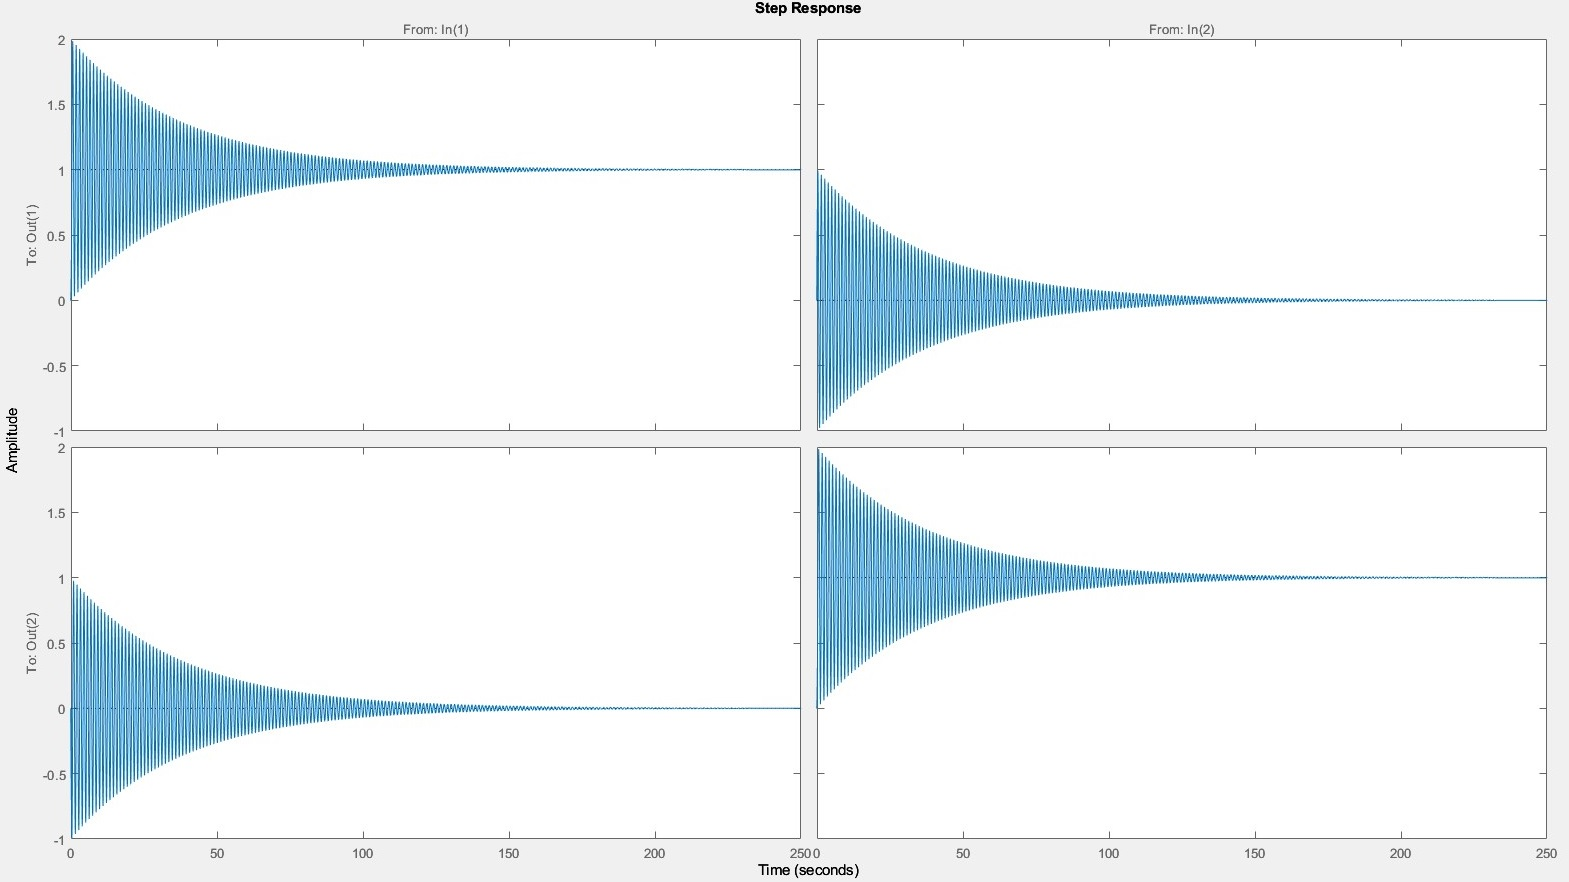
\includegraphics[width=0.9\linewidth]{inc/task1_step}}
	\caption{Отклик на функцию Хевисайда}
	\label{task1_step}
\end{figure}

\begin{figure}[!h]
	\center{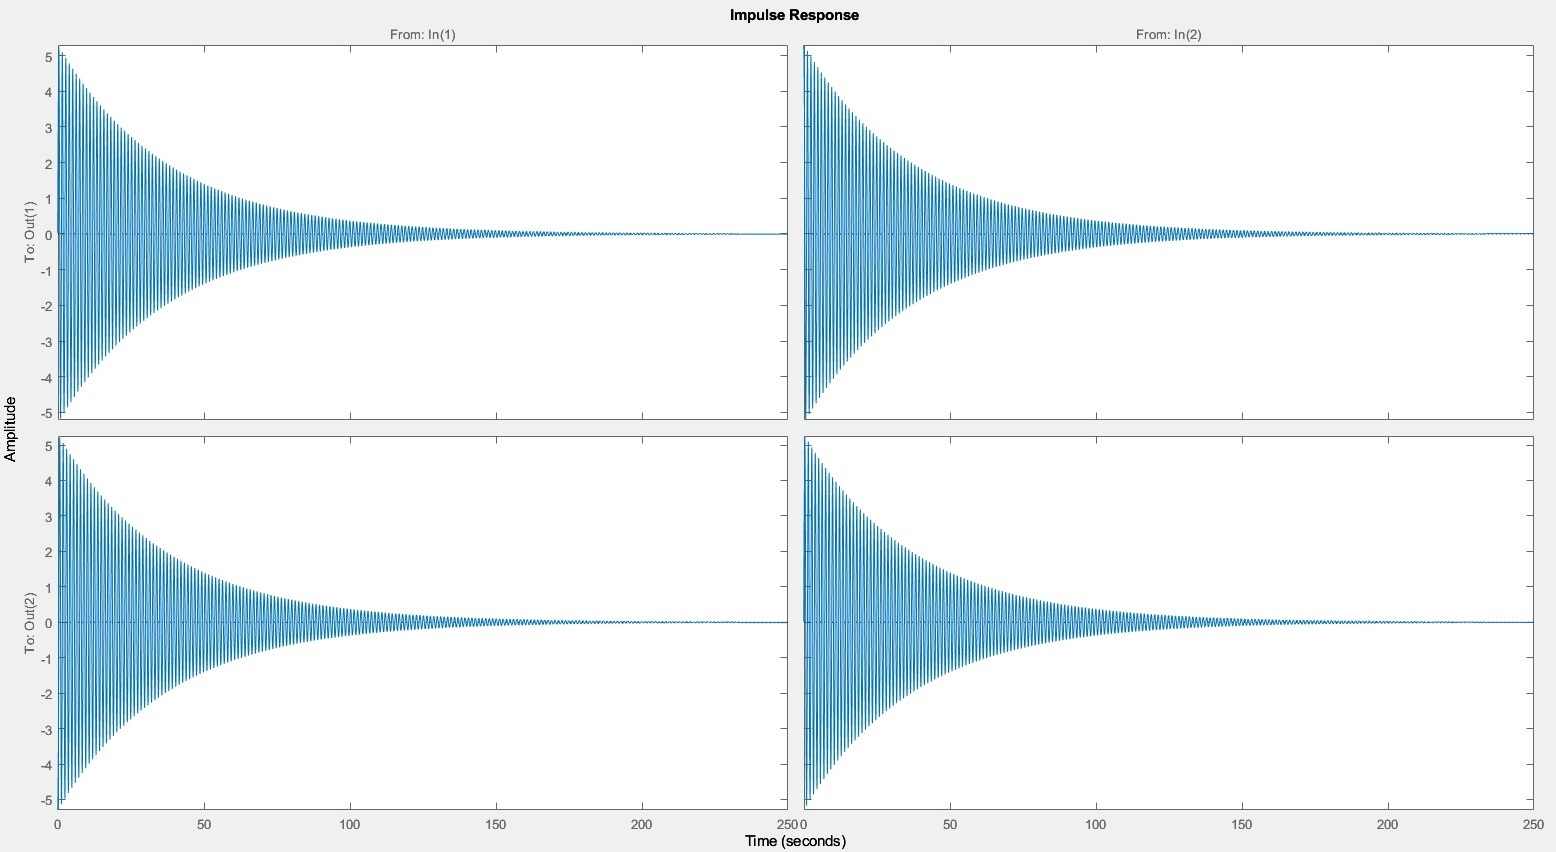
\includegraphics[width=0.9\linewidth]{inc/task1_impulse}}
	\caption{Отклик на единичный импульс}
	\label{task1_impulse}
\end{figure}

% Отобразить в отчете графики, что по осям?

\newpage
\textbf{Часть 2}

Затем проверим нуль-пространство матриц G систем из первой части, их детерминант, характеристическое уравнение, его корни.

Результатом null(G) является пустая матрица. Детерминант равен 28.0560. Характеристическое уравнение имеет коэффициенты 1.0000, 0.0530 и 28.0560, а корни характеристического полинома p равны -0.0265 + 5.2967i и -0.0265 - 5.2967i.

Теперь вычислим переходную матрицу системы используя символьную переменную syms t:

Элемент матрицы (0 0):
\\
\noindent $\frac{\exp(\pi t (- 843/100000 - 843i/500))}{2} + \frac{\exp(\pi t (- 843/100000 + 843i/500))}{2}$

Элемент матрицы (0 1):
\\
\noindent $-\frac{\exp(\pi t (- 843/100000 - 843i/500))\cdot 1i}{2} + \frac{\exp(\pi t (- 843/100000 + 843i/500))\cdot 1i}{2}$

Элемент матрицы (1 0):
\\
\noindent $\frac{\exp(\pi t (- 843/100000 - 843i/500))\cdot 1i}{2} - \frac{\exp(\pi t (- 843/100000 + 843i/500))\cdot 1i}{2}$

Элемент матрицы (1 1):
\\
\noindent $\frac{\exp(\pi t (- 843/100000 - 843i/500))}{2} + \frac{\exp(\pi t (- 843/100000 + 843i/500))}{2}$

Вся матрица:
\\ \\
\noindent $\begin{bmatrix}
	\frac{\exp(\pi t (- 843/100000 - 843i/500))}{2} + & -\frac{\exp(\pi t (- 843/100000 - 843i/500))\cdot 1i}{2} + \\
	+ \frac{\exp(\pi t (- 843/100000 + 843i/500))}{2} & + \frac{\exp(\pi t (- 843/100000 + 843i/500))\cdot 1i}{2} \\
	\frac{\exp(\pi t (- 843/100000 - 843i/500))\cdot 1i}{2} - & \frac{\exp(\pi t (- 843/100000 - 843i/500))}{2} + \\
	- \frac{\exp(\pi t (- 843/100000 + 843i/500))\cdot 1i}{2} &  + \frac{\exp(\pi t (- 843/100000 + 843i/500))}{2} \\
\end{bmatrix}$
\\

Матричная экспонента используется для анализа и решения линейных систем с постоянными коэффициентами. Она может быть использована для предсказания поведения системы.

\newpage
\textbf{Часть 3}

Для начала выведем наш сигнал из ЛР1 (рис. \ref{task3_signal}):
\begin{figure}[!h]
	\center{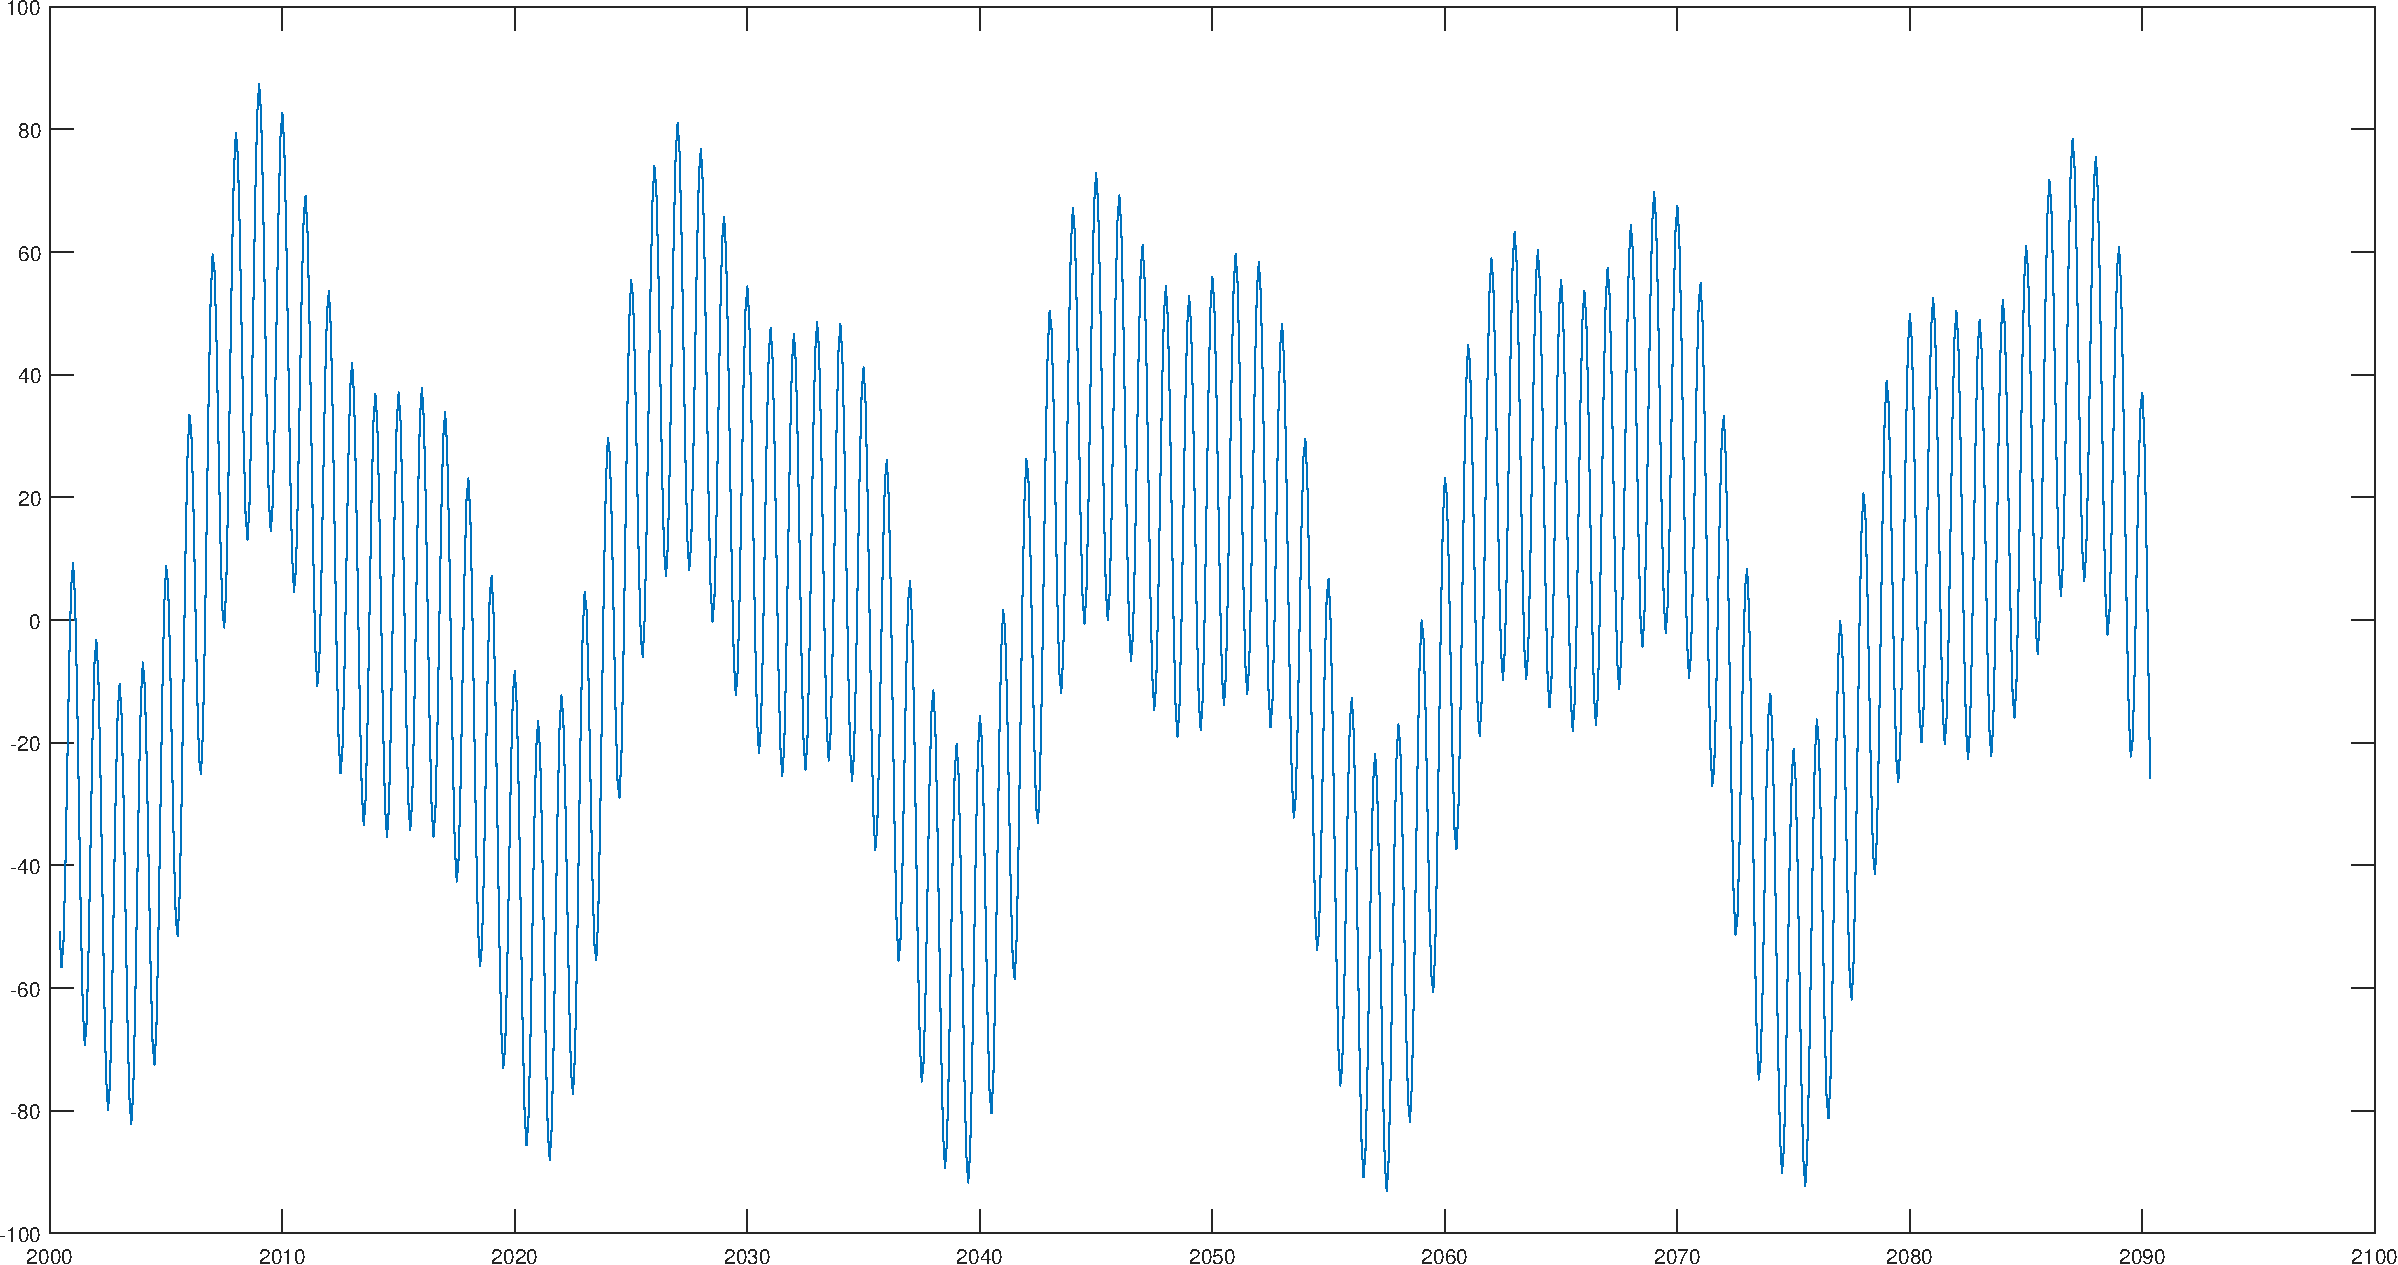
\includegraphics[width=1\linewidth]{inc/task3_signal}}
	\caption{Сигнал из ЛР1}
	\label{task3_signal}
\end{figure}

В текущем сигнале шаг равен месяцу. Проинтерполируем с помощью функции interp1, сгустив точки с семплингом 6 часов. Возьмем его в смеси с шумом примерно равной с ним амплитуды (рис. \ref{task3_noise}-\ref{task3_signal_noise}):

\begin{figure}[!h]
	\center{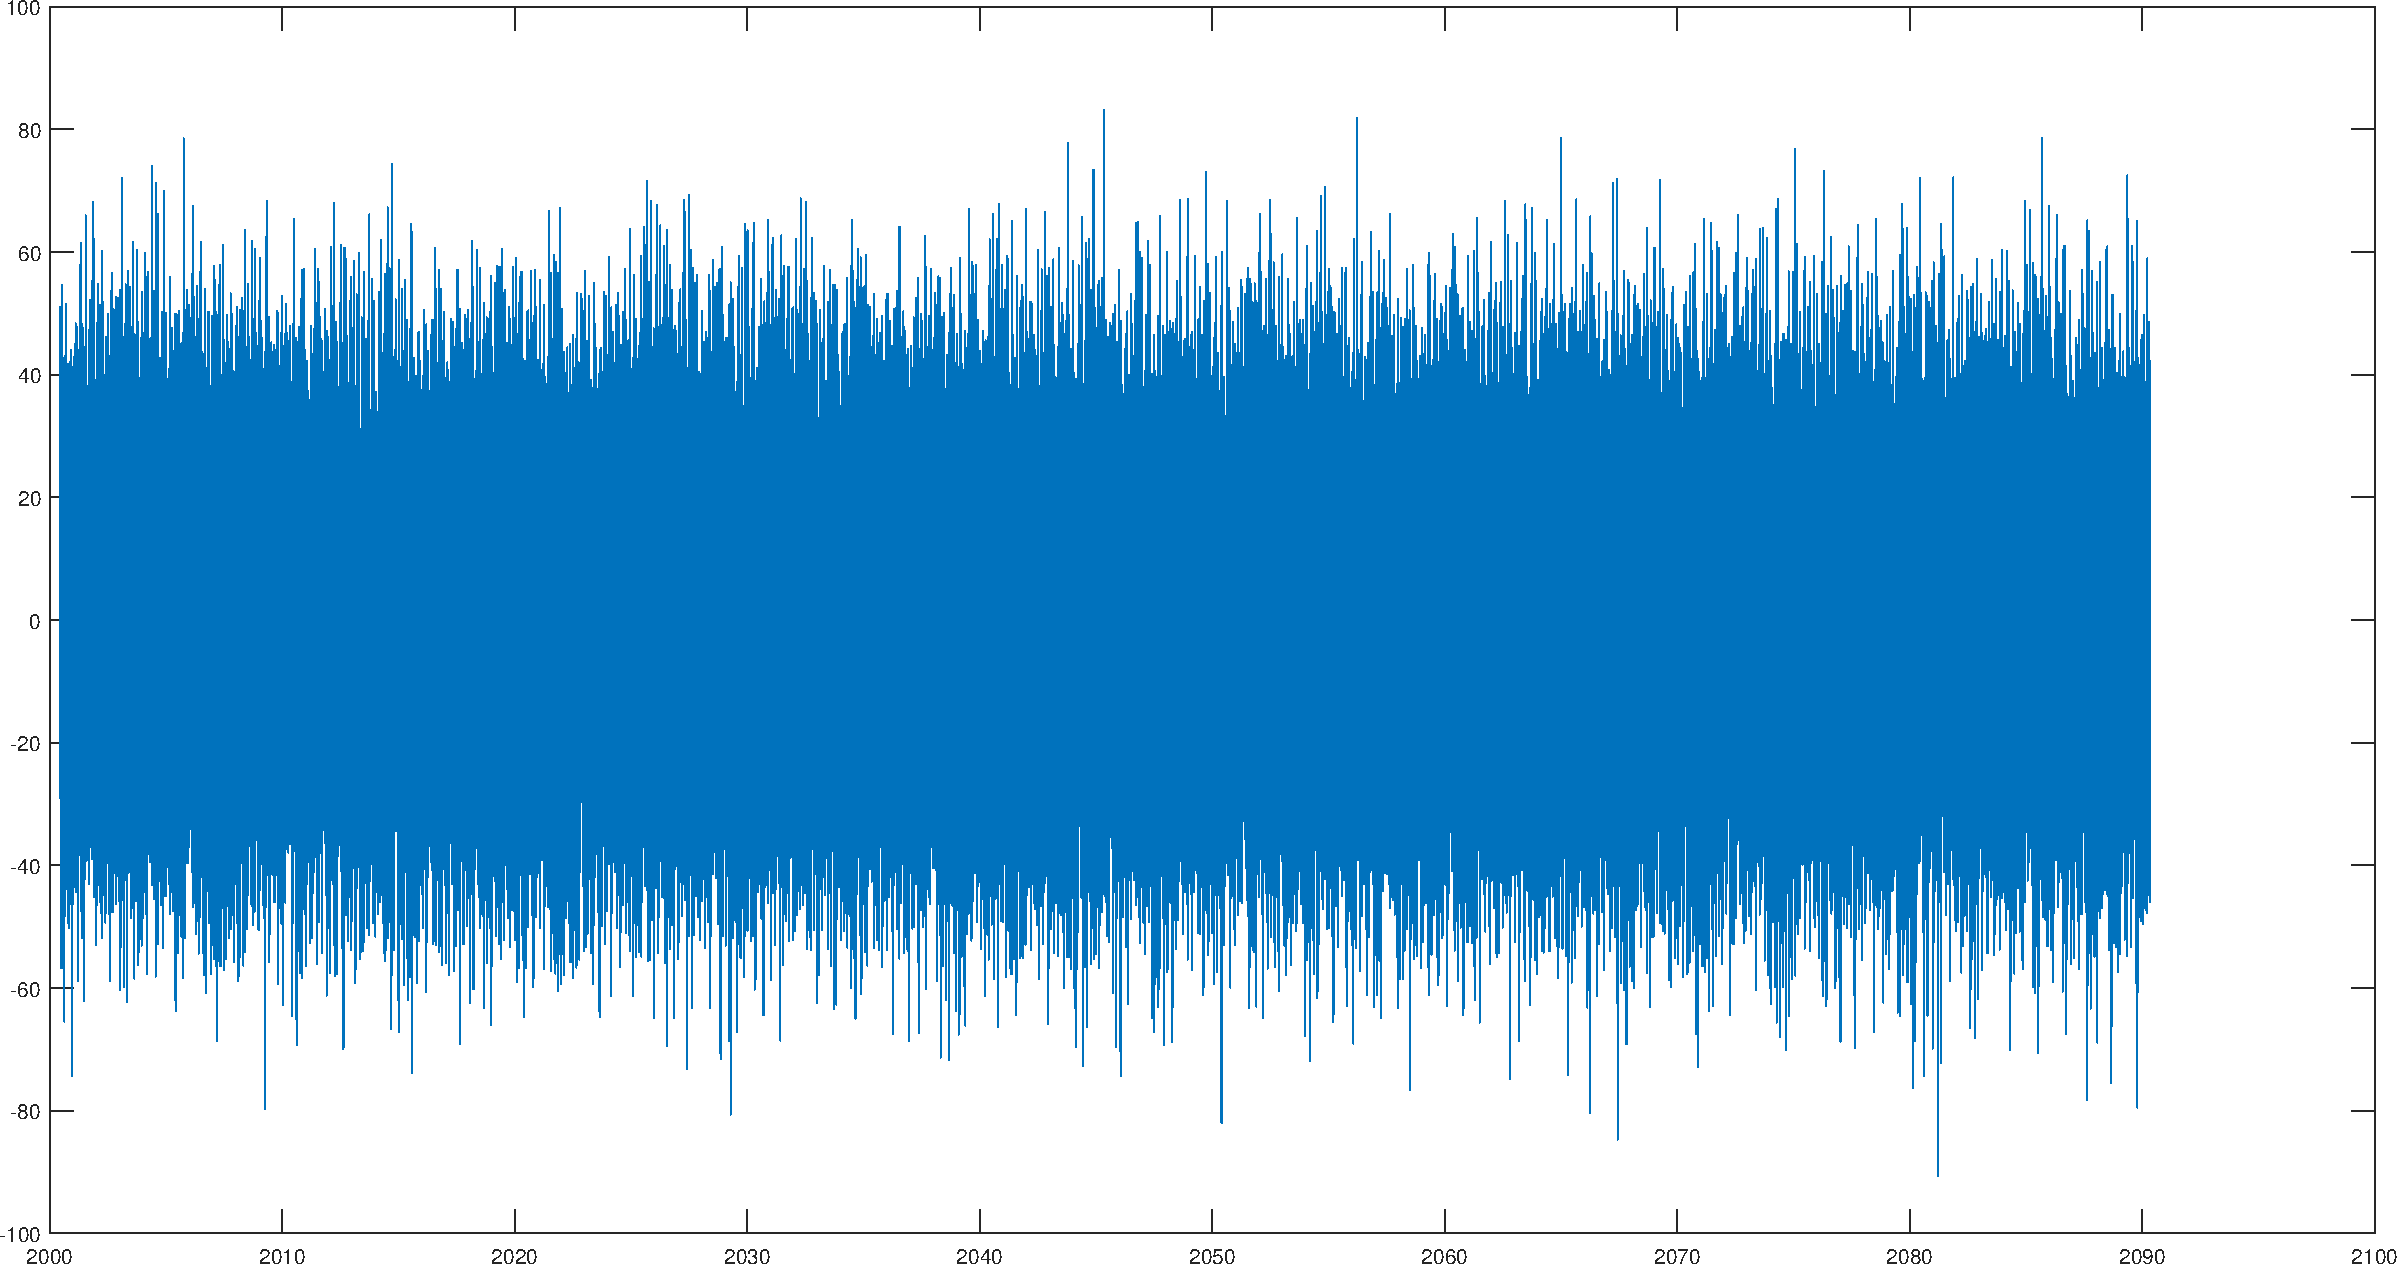
\includegraphics[width=1\linewidth]{inc/task3_noise}}
	\caption{Шум}
	\label{task3_noise}
\end{figure}

\newpage
\begin{figure}[!h]
\center{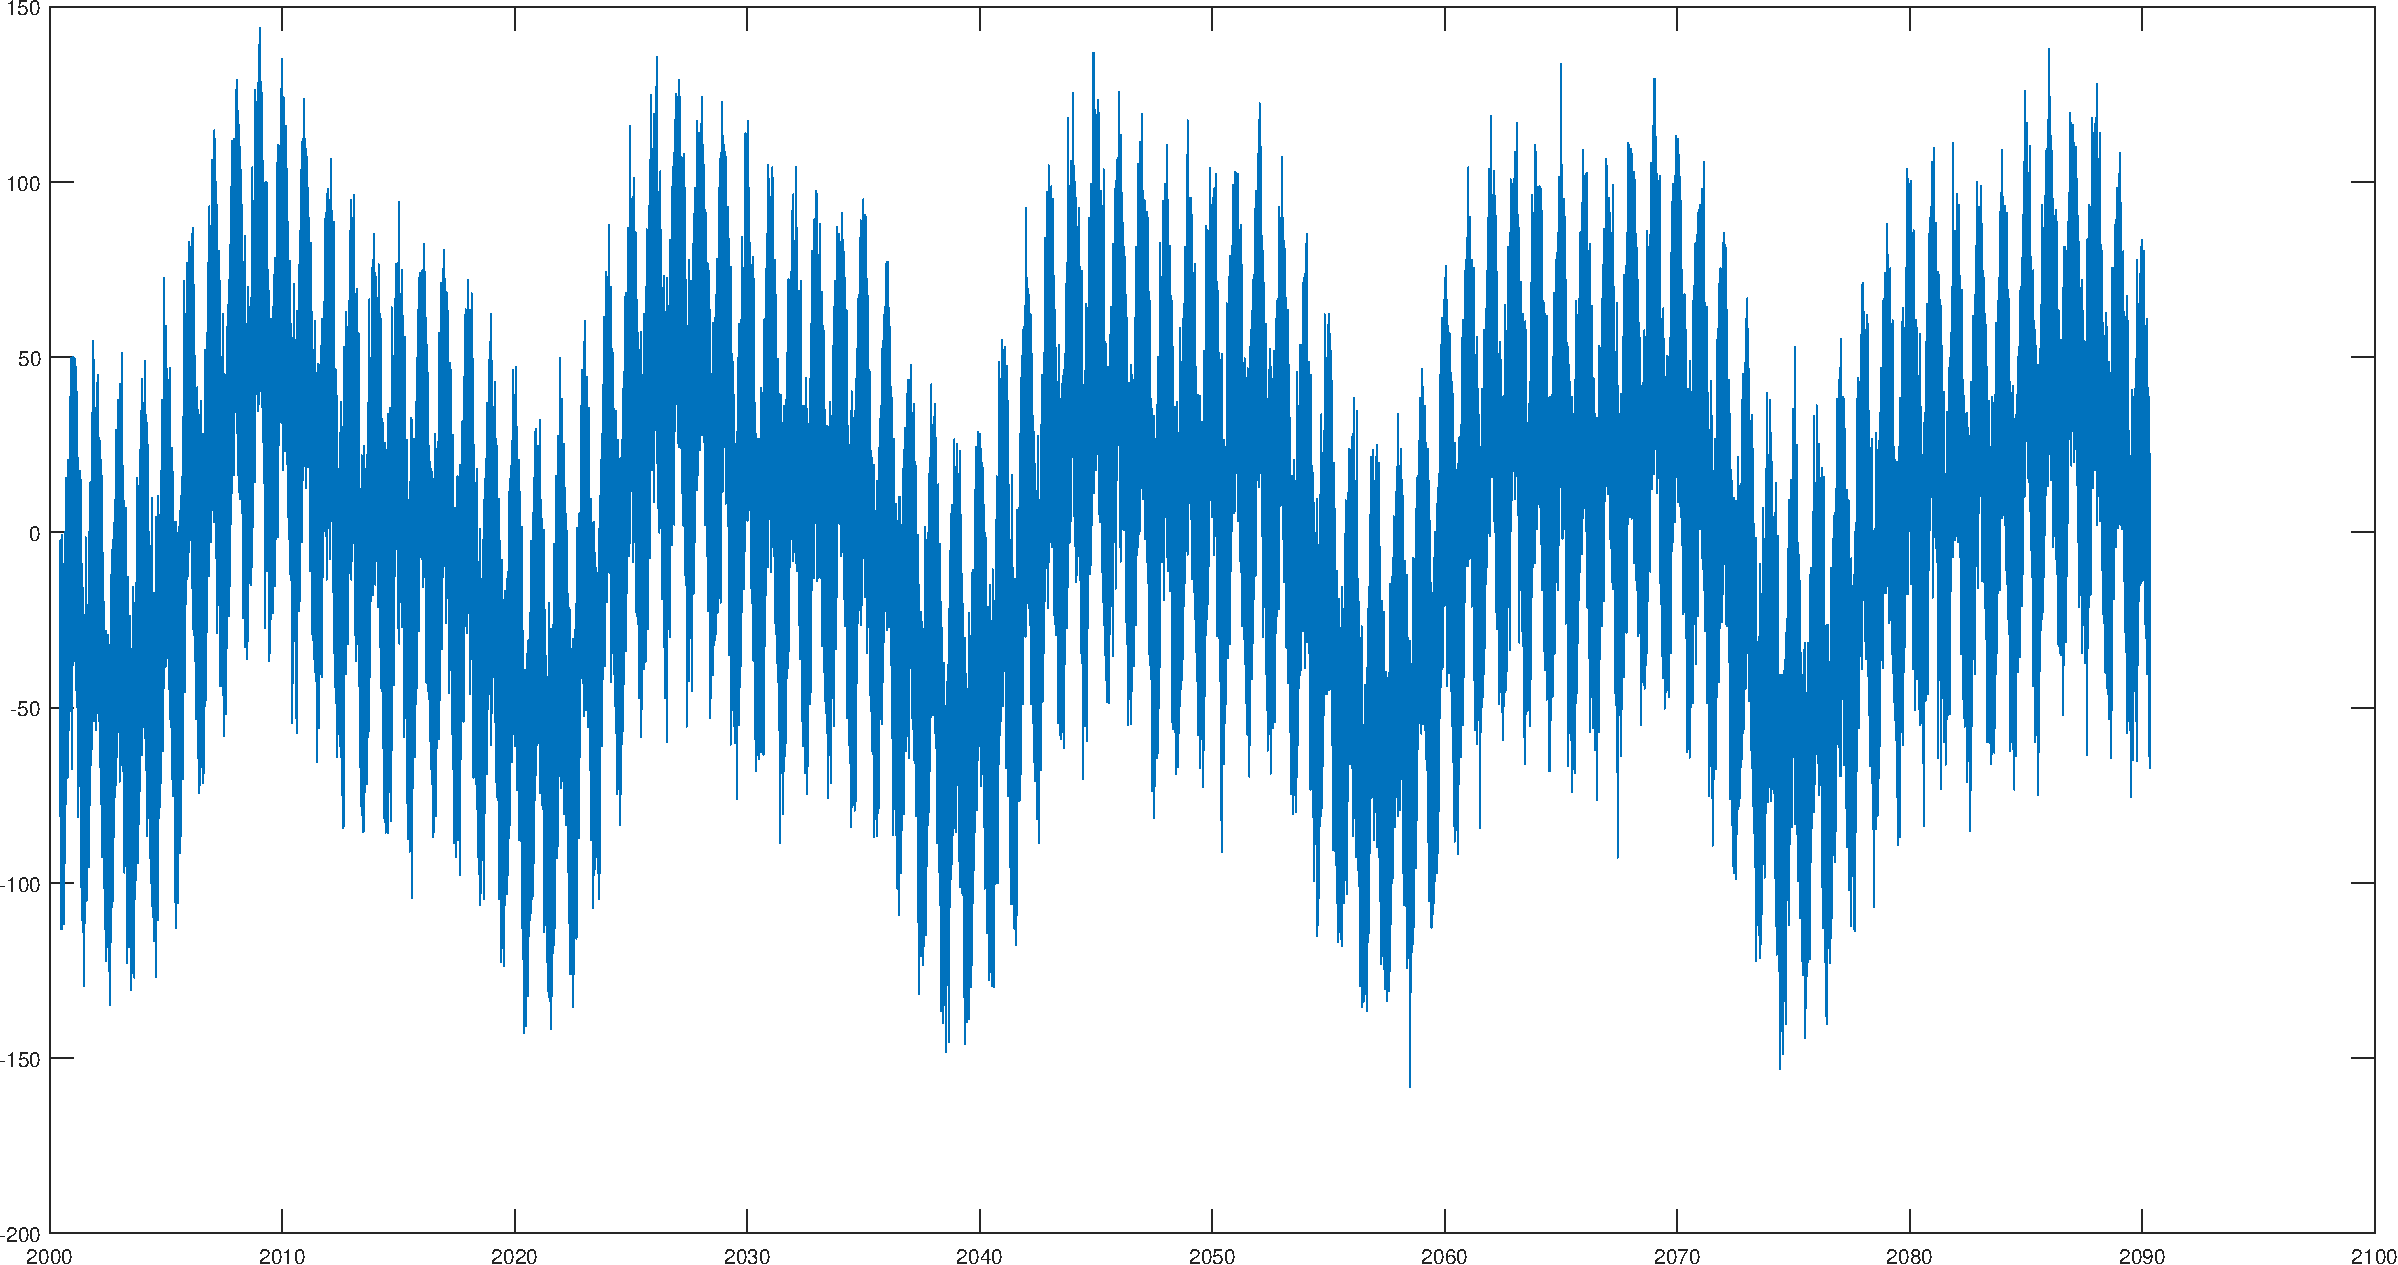
\includegraphics[width=1\linewidth]{inc/task3_signal_noise}}
\caption{Сигнал с шумом}
\label{task3_signal_noise}
\end{figure}

Построим СПМ (рис. \ref{task3_psd}):
\begin{figure}[!h]
	\center{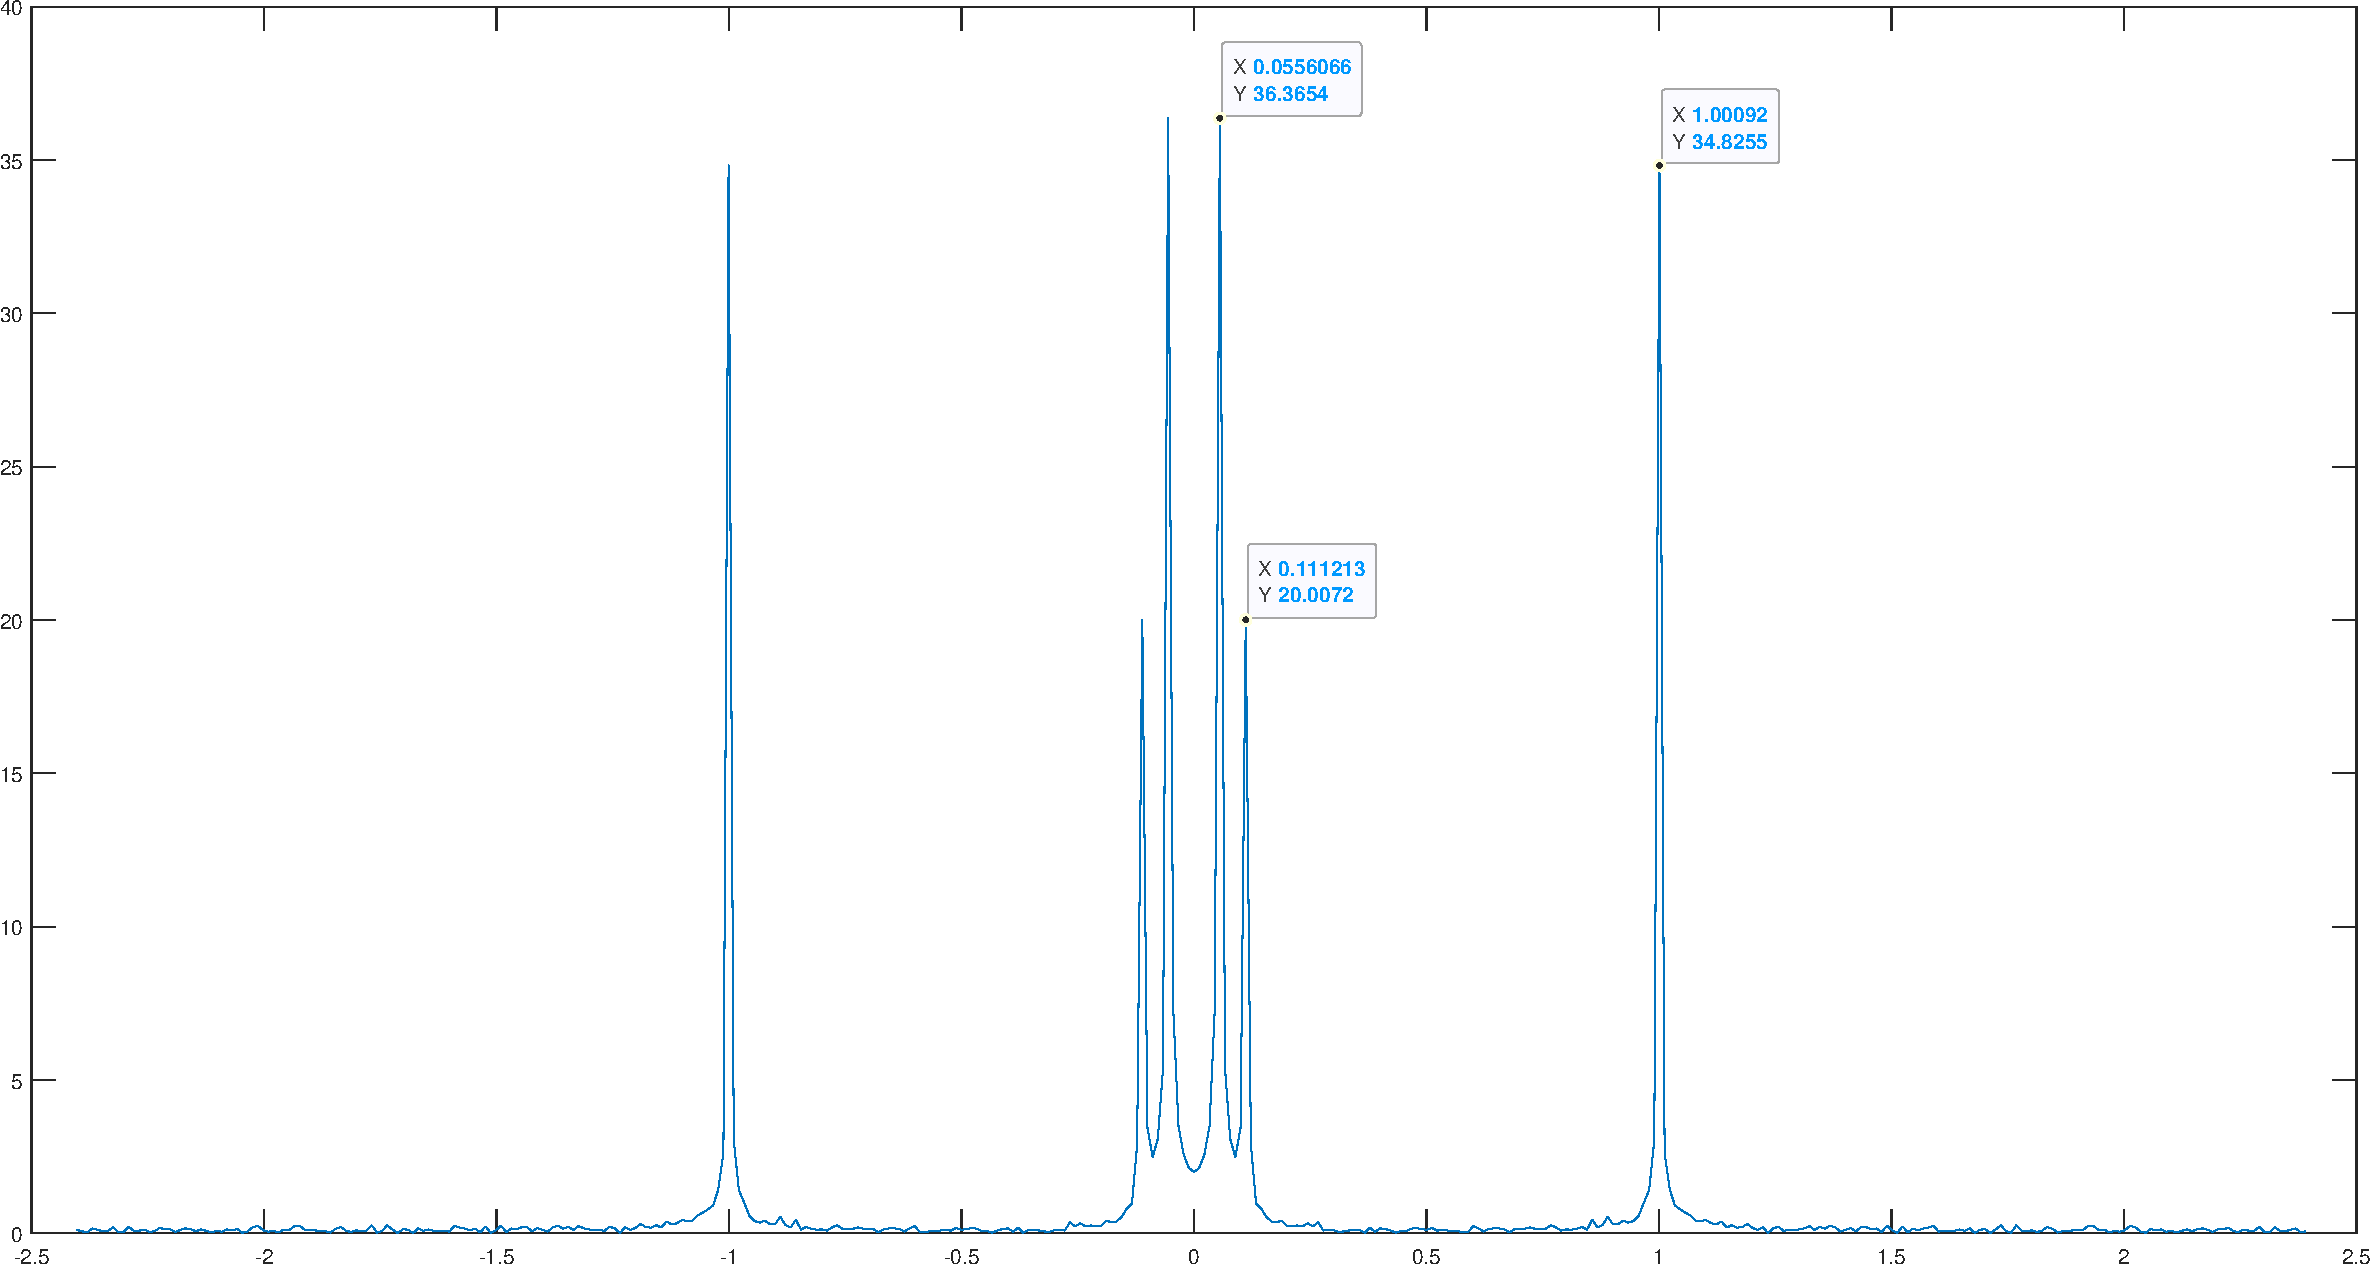
\includegraphics[width=1\linewidth]{inc/task3_psd}}
	\caption{СПМ}
	\label{task3_psd}
\end{figure}

\noindent По пиковым значениям можно проверить линейные частоты изначальных гармоник: 

\noindent $1 \text{ цикл в год, } \frac{1}{1} = 1 \text{, что соответствует гармонике с периодом 1 год}$

\noindent $0.(1) \text{ цикл в год, } \frac{1}{0.111111} \approx 9\text{, что соответствует гармонике с периодом 8.86 год}$

\noindent $0.0(5) \text{ цикл в год, } \frac{1}{0.055556} \approx 18\text{, что соответствует гармонике с периодом 18.6 год}$

\noindent А также амплитуды: $\sim 20, 36$ и $38$

\newpage

Протестируем динамическую систему, запустив функцию lsim подав на оба канала signal+noise, считая начальным состоянием (0,0) и шагом 6 часов, но только для первых 30К точек, $\sim 21$ год (рис. \ref{task3_lsim}):

\begin{figure}[!h]
	\center{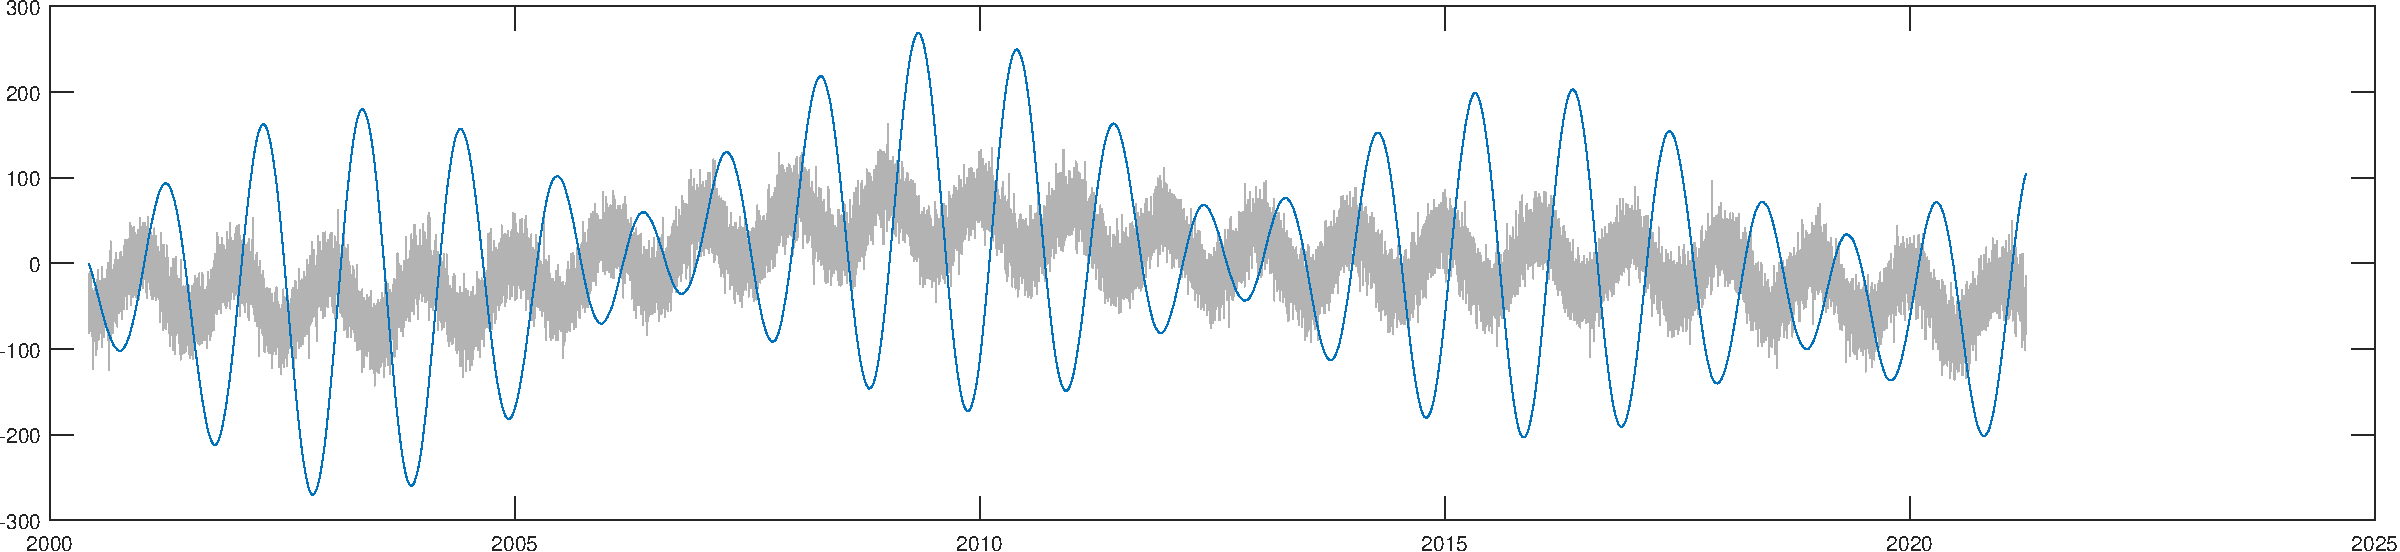
\includegraphics[page=1,width=1\linewidth]{inc/task3_lsim}}
	\center{\includegraphics[page=2,width=1\linewidth]{inc/task3_lsim}}
	\caption{Результат lsim}
	\label{task3_lsim}
\end{figure}

На первом графике рисунка \ref{task3_lsim} серым изображен сигнал с шумом, а на втором они же по отдельности. Синим нарисован отклик системы на входной сигнал. Как видно, он более сглаженный, чем исходный сигнал, а также не содержит высокочастотных компонентов и не подвержен влиянию шумов.

Кроме этого наблюдается задержка отклика. Для  высокочастотных сигналов она более заметная, поскольку система может не успевать адекватно реагировать на быстрые изменения в сигнале. Низкочастотные сигналы, напротив, могут быть лучше учтены системой, и задержка будет менее критичной.

\end{document}